\documentclass[letterpaper,12pt]{article}
\usepackage{tabularx} % extra features for tabular environment
\usepackage{amsmath}  % improve math presentation
\usepackage{graphicx} % takes care of graphic including machinery
\usepackage[margin=0.95in,letterpaper]{geometry} % decreases margins
\usepackage{cite} % takes care of citations
\usepackage[titletoc,title]{appendix} % takes care of appendices
\usepackage{listings} % code representation
\usepackage{pdflscape}
\usepackage{csquotes} % for quoting existing work
\usepackage{color} % defines colours for code listings
\usepackage{comment} % allows for block of comments
\usepackage{gensymb} % degree symbol
\usepackage[cc]{titlepic}  % allows a pic to be included in the title page
\usepackage[final]{hyperref} % adds hyper links inside the generated pdf file

% style code listings
\definecolor{codegreen}{rgb}{0,0.6,0}
\definecolor{codegray}{rgb}{0.5,0.5,0.5}
\definecolor{backcolour}{rgb}{0.95,0.95,0.92}
\lstdefinestyle{mystyle}{
    backgroundcolor=\color{backcolour},   
    commentstyle=\color{codegreen},
    keywordstyle=\color{blue},
    numberstyle=\tiny\color{codegray},
    basicstyle=\footnotesize,
    breakatwhitespace=false,         
    breaklines=true,                 
    captionpos=b,                    
    keepspaces=true,                 
    numbersep=5pt,                  
    showspaces=false,                
    showstringspaces=false,
    showtabs=false,                  
    tabsize=4
}
\lstset{style=mystyle}

\begin{document}

\title{
    CS5011 Artificial Intelligence Practice\\Assignment 4 Report\\
    \begin{large}
    University of St Andrews - School of Computer Science
    \end{large}
}
\titlepic{
\includegraphics[width=0.3\linewidth]{report/figures/st-andrews-logo.jpeg}}
\author{Student ID: 150014151}
\date{20th December, 2019}
\maketitle
\newpage

\tableofcontents
\newpage


% --------------------------------------- 1 - INTRODUCTION ------------------------------------------ 

\section{Introduction}
\label{sec:introduction}

The following requirements were attempted:
\begin{itemize}
    \item Basic Agent:
    \begin{itemize}
        \item Multilayer feedforward neural network.
        \item Data encoding and training/testing split.
        \item Grid search algorithm for determining optimal hyperparameters.
    \end{itemize}
    \item Intermediate Agent:
    \begin{itemize}
        \item CLI text-based interface.
    \end{itemize}
    \item Additional Features:
    \begin{itemize}
        \item Training result visualisation in plots and heatmaps.
    \end{itemize}
        
\end{itemize}

\subsection{Installation}

Create a virtual environment for the project and activate it:

\begin{lstlisting}
virtualenv ~/Environments/A4
source ~/Environments/A4/bin/activate
\end{lstlisting}

Once you have the virtual environment activated, \textit{cd} into the project directory and install the requirements needed to run the app:

\begin{lstlisting}
pip install -r requirements.txt
\end{lstlisting}

\subsection{Usage}

To compile the program, navigate to the \textit{A4src} directory and run the following command:

\begin{lstlisting}
python A4Main.py [-h] -a <AGENT> -c <CSV> [-g] [-d]
\end{lstlisting}

where:

\begin{itemize}
    \item \textit{AGENT} is the type of agent to run: \textit{[Bas, Int, Adv]}:
    \begin{itemize}
        \item \textit{Bas}: Train and test the neural network with the optimal parameters, or run the Grid Search algorithm to determine the optimal parameters.
        \item \textit{Int}: CLI text-based application to submit a new ticket and predict to which response team it should go.
        \item \textit{Adv}: todo.
    \end{itemize}
    \item \textit{CSV} is the CSV file containing the data used to train/test the data.
    \item \textit{-g}: flag set to run the grid search algorithm.
    \item \textit{-d}: flag set to enter debug mode, printing more statements to the command line.
    \item \textit{-h}: flag for help on how to use the agent.
\end{itemize}

\paragraph{Examples}

Here are a few examples that can be used to run the program:

\begin{itemize}
    \item ``\textit{python A4Main.py -a Bas -c tickets -d}'' to train/test the neural network.
    \item ``\textit{python A4Main.py -a Bas -c tickets -g}'' to run the grid search algorithm.
    \item ``\textit{python A4Main.py -a Int -c tickets}'' to submit a new ticket through the CLI text-based interface
    \item ``\textit{python A4Main.py -h}'' for help on how to run the agent.
\end{itemize}

\subsection{Tools Used}

\begin{itemize}
    \item Scikit\footnote{Scikit: \url{https://scikit-learn.org}} and related Python libraries (e.g. NumPy\footnote{NumPy: \url{https://numpy.org/}}, Pandas\footnote{Pandas: \url{https://pandas.pydata.org/}}, Matplotlib\footnote{Matplotlib: \url{https://matplotlib.org/}}).
    \item PyCharm\footnote{PyCharm: \url{https://www.jetbrains.com/pycharm/}}: an IDE developed by JetBrains to write Python code with support for some of the above libraries.
    \item Git and GitHub: to back and version control the code.
    \item PEP8\footnote{PEP8: \url{https://www.python.org/dev/peps/pep-0008/}} coding guidelines and docstring followed throughout the entire code.
\end{itemize}

% -------------------------- 2 - DESIGN - IMPLEMENTATION - EVALUATION -------------------------------

\clearpage
\section{Design, Implementation \& Evaluation}
\label{sec:design-implementation-evaluation}

\subsection{Design: PEAS Model}

This section defines the PEAS model for a ticketing routing-based agent that uses a multilayer feedforward neural network in order to ultimately learn how to make smart predictions for the appropriate response team of future tickets.

\paragraph{Performance measure}\label{sec:performance-measures} The basic agent can be evaluated by the efficiency of the training step based on the number of epochs required to train to a certain target error, and the testing accuracy using a confusion matrix. The intermediate agent can be assessed by the number of questions to make a prediction and their correctness can also be measured.

\paragraph{Environment} This is a single-agent and fully-observable environment represented by a neural network and the text-based interface used to interact with a user logging a new ticket. Additionally, it can be said that the basic agent environment is deterministic (the next state is determined by the current state and the action executed) and stochastic for the intermediate agent (user input is unknown), according to the definitions set by Russell \& Norvig in \textit{Artificial intelligence: a modern approach} \cite{russell2016artificial}.

\paragraph{Actuators} The agent may accept input and target data it can learn from by backpropagating the calculated error between the input and target data in order to adjust the weights of the neural network (also known as Stochastic Gradient Descent). It may also predict an output based on unseen data.

\paragraph{Sensors} The basic agent is always aware of the environment and can calculate feedback error based on input and target data, while the intermediate agent can receive responses to questions by interacting with a human user.

% ----------------------------------

\subsection{Implementation}

\subsubsection{Project Structure}

The project is divided in three main sections:

\begin{itemize}
    \item The \textit{agents} module, containing functions to implement the execution of flow of each agent.
    \item The \textit{neural\_network} module, which contains classes to create and manipulate a multilayered perceptron, a data encoder/processor and the grid search algorithm.
    \item The \textit{main} section, containing the program's entry point \textit{A4Main.py} for parsing the command line arguments, global configuration settings in \textit{config.py} and printing methods in \textit{helpers.py}.
\end{itemize}

The \textit{data} directory stores the CSV data, the \textit{neural\_networks} directory the trained neural nets in \textit{``*.joblib''} format, and the \textit{results} directory the output of the grid search algorithm.

% ----------------------------------

\subsubsection{Neural Network Training \& Testing (Basic Agent)}

The basic agent takes a CSV file as input used for training and testing. It creates a new instance of the custom \textit{DataProcessor} class, which contains functions for parsing the CSV file (retrieving tags and categories), splitting the data between inputs and targets, and encoding/decoding it. The input data is encoded in either 0s or 1s, while the target data is encoded using one-hot encoding. Figure \ref{fig:data_encoding} depicts how the data is split and encoded.

\begin{figure}[h] 
\centerline{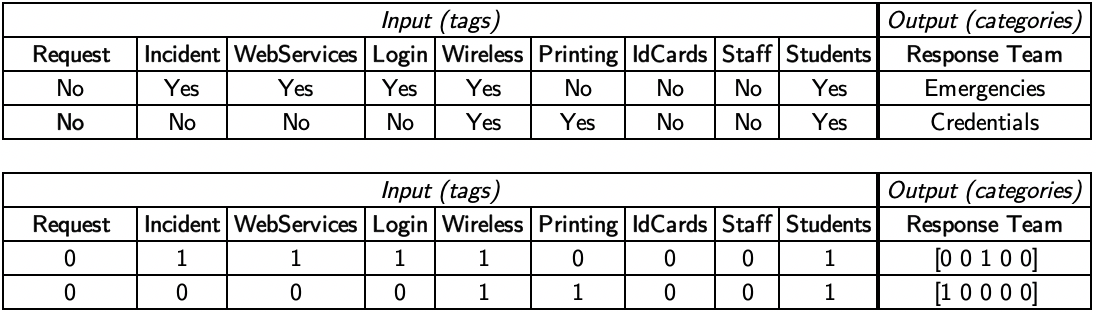
\includegraphics[width=\textwidth]{report/figures/data_encoding.png}}
\caption{\label{fig:data_encoding}todo.}
\end{figure}

The data must be fed to the neural network in binary form. Therefore, one-hot encoding is chosen for the target categories as there are only five in total, which suits the sparse representation of the data. Only a single digit may have the value 1 in one-hot encoding, while the others remain at value 0. The one-hot encodings of the target data can be seen in Figure \ref{fig:one_hot_encoding}.

\begin{figure}[h] 
\centerline{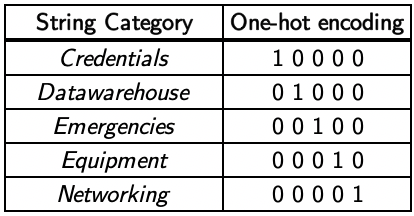
\includegraphics[width=0.4\textwidth]{report/figures/one_hot_encoding.png}}
\caption{\label{fig:one_hot_encoding}todo.}
\end{figure}

Once the data is encoded, an instance of the custom \textit{MultiLayerPerceptron} class is created, containing functions to split the training/testing data, training \& testing the neural network, displaying results and saving the network with the trained weights. The class uses \textit{Scikit}'s \textit{MLPClassifier}\footnote{Scikit MLPClassifier: \url{https://scikit-learn.org/stable/modules/generated/sklearn.neural_network.MLPClassifier.html}} to implement the neural network. The class instantiates with default hyperparameters for the neural network, which can be overwritten when creating a new \textit{MultiLayerPerceptron} (see Listing below).

\begin{lstlisting}[language=Python]
class MultiLayerPerceptron:
    def __init__(self, name, input_data, target_data, hidden_layers_size=(15,), solver="adam", activation_function="logistic", learning_rate_init=0.6, momentum=0.9, optimisation_tolerance=0.0001, num_iterations_no_change=1000, max_iterations=10000, verbose=config.debug):
\end{lstlisting}

An 80\%/20\% split is used for the training/testing data sets, with equal category distribution maintained between the training and testings sets, which is ensured through the use of the \textit{stratify} option in Scikit's \textit{train\_test\_split} function\footnote{Scikit train\_test\_split: \url{https://scikit-learn.org/stable/modules/generated/sklearn.model_selection.train_test_split.html}}. Indeed, because the data has 250 entries (including 50 for each of five outputs), the testing set will have 10 entries for each of the five categories.\\

The actual training is done with the \textit{fit} function, with the error loss plotted with regards to the number of epochs; while the testing is performed using the \textit{predict} and \textit{predict\_proba} functions and its accuracy visualised with a confusion matrix. These results can be seen in Section EVALUATION.

% ----------------------------------

\subsubsection{CLI Text-Based Ticketing-Routing Agent (Intermediate Agent)}

todo

% ----------------------------------

\subsubsection{Advanced}

todo


% ----------------------------------

\subsection{Evaluation}
\label{sec:evaluation}

todo

\textit{Design, Implementation \& Evaluation Section word count: \underline{XXXX}}

% -------------------------------------- 3 - TEST SUMMARY ------------------------------------------ 
\section{Test Summary}
\label{sec:test-summary}

todo


% -------------------------------------- APPENDICES ------------------------------------------ 
\begin{appendices}

\clearpage
\bibliographystyle{plain}
\bibliography{bibliography}

% ------------------------

\clearpage
\section{UML Class Diagram}
\label{sec:appendix-uml-class-diagram}

The UML Class Diagrams of the code, generated by the yWorks \cite{yworks} plugin in the IntelliJ IDEA IDE.

todo

% ------------------------

\clearpage
\section{Project File Structure}
\label{sec:appendix-project-file-structure}

todo

% ------------------------

\end{appendices}
\end{document}